\documentclass{article}
\usepackage[utf8]{inputenc}
%%Para esconder subsecciones en el índice:
%\setcounter{tocdepth}{1}


%Microtype
\usepackage[activate={true,nocompatibility},final,tracking=true,kerning=true,spacing=true,factor=1100,stretch=10,shrink=10]{microtype}
% activate={true,nocompatibility} - activate protrusion and expansion
% final - enable microtype; use "draft" to disable
% tracking=true, kerning=true, spacing=true - activate these techniques
% factor=1100 - add 10% to the protrusion amount (default is 1000)
% stretch=10, shrink=10 - reduce stretchability/shrinkability (default is 20/20)
\microtypecontext{spacing=nonfrench}
  \usepackage{pgfplots}
  \pgfplotsset{compat=newest}
  %% the following commands are needed for some matlab2tikz features
  \usetikzlibrary{plotmarks}
  \usetikzlibrary{arrows.meta}
  \usepgfplotslibrary{patchplots}
  \usepackage{grffile}
  %% Language and font encodings
\usepackage[english, spanish]{babel}
\usepackage[utf8]{inputenc}
\usepackage[T1]{fontenc}


% Sets page size and margins
\usepackage[a4paper,top=3cm,bottom=2cm,left=2.7cm,right=2.7cm,marginparwidth=1.75cm]{geometry}
%Para los gráficos
\definecolor{mycolor1}{rgb}{0.00000,0.44706,0.74118}%
\definecolor{mycolor2}{RGB}{255,165,0}%
\definecolor{rojo}{RGB}{255,0,0}%
\definecolor{verde}{RGB}{50,205,90}%
\definecolor{azulfrancia}{rgb}{0.00000,0.44706,0.74118}%
\definecolor{boston}{rgb}{0.8, 0.0, 0.0}
\usepackage{float}

%Tabla
\usepackage{booktabs}% http://ctan.org/pkg/booktabs
\usepackage{xcolor}
\usepackage{graphicx}
\usepackage{colortbl}
\usepackage{array}
\usepackage{pifont}
\usepackage{tabularx}

%% Useful packages
\usepackage{parskip}
\usepackage{pdflscape}
\usepackage{amsmath}
\usepackage{graphicx}
\usepackage[makeroom]{cancel}
\usepackage{tikz}
\usepackage{amssymb}
\usepackage[version=4]{mhchem}
\usepackage{textcomp}
\usepackage{gensymb}
\usepackage{circuitikz}
\usepackage{multicol}
\usepackage{caption}
\usepackage[colorinlistoftodos]{todonotes}
\usepackage[colorlinks=true, allcolors=black]{hyperref}
\usepackage[
backend=biber, style=ieee
]{biblatex}
\addbibresource{bibliografia.bib}

  %% you may also want the following commands
  %\pgfplotsset{plot coordinates/math parser=false}
  %\newlength\figureheight
  %\newlength\figurewidth
\usepackage{verbatim}
\usepackage[nodisplayskipstretch]{setspace}
\setstretch{1.2}
\usepackage{multicol}
\usepackage{caption}
\usepackage{subcaption}
\usepackage{chemfig}
\usepackage{geometry}
\usepackage{enumitem}
\usepackage{multirow}
\title{Análisis FMEA}
\author{Nicolás Goldman}
\date{March 2020}

\begin{document}

\maketitle

\section{Introduction}
En esta sección se analiza, de acuerdo a sus características durante operación normal, el grado de robustez del Sistema Primario de Refrigeración y, por lo tanto, el nivel de   confiabilidad   en   la   capacidad   de  remover   la   potencia   térmica  del   Sistema   de Resistencias  y  transferirlo  a  través  los  Generadores  de  Vapor  al  fluido  del  Sistema Secundario.

Para llevar a cabo dicho análisis se emplea la metodología de evaluación de riesgo FMEA (Failure Mode Effect Analysis), cuyo propósito es caracterizar las distintas causas de fallas,  mediante  el  Número  Prioritario  de  Riesgo  (RPN),  el  cual  se  estima  mediante  los índices Severity (Severidad), Occurrence (Frecuencia) y Detection (Detección).

Las funciones del circuito se pueden definir en términos de variables medibles como la circulación de un caudal de refrigerante, con ciertos valores de presión y temperatura. En consecuencia, los modos de falla son:
\begin{enumerate}
    \item Caudal de refrigerante fuera del rango de diseño.
    \item Temperatura de refrigerante fuera del rango de diseño.
    \item Presión del fluido refrigerante fuera del rango de diseño.
    \item Conductividad del fluido refrigerante excesiva
\end{enumerate}

Los componentes de este sistema son:
\begin{itemize}
    \item Sistema de bombas de baja presión
    \item Generador de Vapor
    \item Condensador de aceite
    \item Sistema de Resistencias de Calefacción
    \item Tanque Presurizado/Expansión
    \item Sistema de Filtros
\end{itemize}
Teniendo  en  cuenta  las  características  de  los  equipos  y  su  operación durante el modo de operación normal, se indican las siguientes causas de falla del sistema:
\begin{table}[H]
\centering
\begin{tabularx}{\textwidth}{XXXXc}
\toprule
\multicolumn{3}{c}{Descripción de unidad} & \multicolumn{2}{c}{Descripción de falla} \\
\midrule
Función & Equipo & Modo de falla & Mecanismo de \newline falla & N° referencia 
\\
\midrule
\multirow{2}{7em}{Compensa la caída de presión debido a fricción en cañerías y equipos} & \multirow{2}{7em}{Sistema de bombeo de baja presión} & \multirow{2}{7em}{Presión fuera del rango de diseño} & Falta de energía eléctrica & 1.a \\
 & & & Falla de los sellos &  1.b \\ \\ \\ \\\midrule
\multirow{2}{7em}{Entrega potencia térmica al fluido refrigerante primario} & \multirow{2}{7em}{Sistema de resistencias calefactoras} & \multirow{2}{7em}{Temperatura fuera del rango de diseño} & Falla eléctrica \newline total & 2.a \\
& & & Baja tensión &  2.b \\ \\ \\ \\\midrule
\multirow{2}{7em}{Mantiene la presión del sistema mediante la presurización del tomo. Regula los cambios de volumen debido a transientes de temperatura} & \multirow{2}{7em}{Tanque presurizador o tanque de expansión} & \multirow{2}{7em}{Presión fuera del rango de diseño} & Ingreso de aire \newline durante el venteo & 3.a \\
 & & & Fuga externa &  3.b\\ \\ \\ \\ \\ \\ \\ \\ \\\midrule
\multirow{2}{7em}{Cede la potencia térmica al sistema secundario} & \multirow{2}{7em}{Generador de vapor} & \multirow{2}{7em}{Temperatura fuera del rango de diseño} & Corrosión y picado en el interior de los tubos & 4.a \\
 & & & Infuga hacia el sistema secundario &  4.b \\\midrule
Remueve material particulado presente en el fluido refrigerante & Sistema de filtros & Conductividad del fluido refrigerante excesiva & Bloqueo del filtro & 5 \\\midrule
Condensa vapor proveniente del sistema de resistencias y del tanque presurizador & Condensador de aceite & Presión fuera del rango de diseño & Ensuciamiento & 6 \\
\bottomrule
\end{tabularx}
\caption{Fallas en el sistema}
\end{table}
\newpage
\subsection{Definición de índices de riesgo}
Se definen a continuación los parámetros que se tendrán en cuenta para caracterizar cada una de las causas de falla de acuerdo al nivel de riesgo e impacto que tienen sobre la especificación del producto.

Como se indicó previamente, el Número Prioritario de Riesgo (RPN) es el producto de tres magnitudes:
\begin{equation}
    RPN = S \cdot O \cdot D
\end{equation}
\begin{itemize}
    \item Severity (S): Da noción de que tan elevado es el impacto en el sistema. A falla más severa, el índice tiene un valor más alto.
    \item Occurence (O): Refiere  a  la  frecuencia  con  la  que  la  falla  puede  ser  tolerada  en  el sistema. A fallas que son poco toleradas, el índice tiene valor un más alto.
    \item Detection (D): Indica la capacidad que tiene el sistema para detectar la causa de la falla. A menor capacidad para detectar la falla, mayor es el índice.
\end{itemize}
La selección de la escala y su significado es subjetiva a las características de los casos analizados.
\begin{table}[H]
\centering
\begin{tabularx}{\textwidth}{cX}
\toprule
Ranking & Nivel \\
\midrule
1 & La falla ocurre y no tiene impacto en el sistema \\
2 & Falla con repercusión menor y tolerable \\
3 & Falla con repercusión elevada. El sistema puede exponerse a daño, puede continuar operando por un tiempo acotado de tiempo hasta que se alcance el nivel de alarma y se tomen medidas correctivas \\
4 & Requiere el cese de operación del circuito y la parada de la planta \\
\bottomrule
\end{tabularx}
\caption{Índice Severity}
\end{table}
\begin{table}[H]
\centering
\begin{tabularx}{\textwidth}{cX}
\toprule
Ranking & Nivel \\
\midrule
1 & Asegurada. Falla evidente \\
4 & Falla escondida. Sin embargo es posible determinar la causa \\
7 & Falla escondida. El origen de la falla es difícil de determinar \\
10 & Falla imposible de detectar \\
\bottomrule
\end{tabularx}
\caption{Índice Detection}
\end{table}
\begin{table}[H]
\centering
\begin{tabularx}{\textwidth}{cX}
\toprule
Ranking & Nivel \\
\midrule
1 & Se permite que ocurra hasta 30 días al año \\
2 & Se permite que ocurra hasta 10 días al año \\
3 & Se permite que ocurra hasta 1 día al año \\
\bottomrule
\end{tabularx}
\caption{Índice Occurence}
\end{table}
Para la determinación de los valores de los índices, se aplican los siguientes criterios:
\begin{itemize}
    \item La severidad del modo de falla de presión es de nivel 4, ya que puede provocar accidentes severos.
    \item La severidad de los modos de falla de temperatura y caudal es de nivel 3, ya que el sistema puede continuar operando a pesar de la falla.
    \item La severidad del modo de falla de la conductividad es de nivel 2, pues produce la corrosión interna de los equipos si no es corregida.
    \item Todas las fallas relacionadas con la corriente eléctrica o con pérdidas al exterior son fácilmente identificables, y su detección es de nivel 1.
    \item El bloqueo del filtro puede notarse por un aumento en la pérdida de carga, y se le asigna una detección de nivel 4.
    \item Todas las fallas ocasionadas por fugas o daños internos se consideran imposibles de identificar, y se les asigna una detección de nivel 10.
    \item En cuanto al nivel de ocurrencia, la falla total de energía eléctrica es inadmisible pues produce una falla total, y tiene nivel 3. La baja de tensión produce una falla intermitente, y se le asigna nivel 1. Todas las demás fallas se pueden considerar parciales y graduales, y se les asigna nivel 2; es decir, se acepta que ocurran con baja frecuencia.
\end{itemize}
\begin{table}[H]
\centering
\begin{tabularx}{\textwidth}{XXccccc}
\toprule
Equipo & Mecanismo de falla & N° referencia & S & O & D & RPN
\\
\midrule
\multirow{2}{7em}{Sistema de bombeo de baja presión} & Falta de energía eléctrica & 1.a & 4 & 3 & 1 & 12 \\
 & Falla de los sellos &  1.b & 4 & 2 & 10 & 80 \\ \\\midrule
\multirow{2}{7em}{Sistema de resistencias calefactoras} & Falla eléctrica \newline total & 2.a & 3 & 3 & 1 & 9 \\
 & Baja tensión &  2.b & 3 & 1 & 1 & 3 \\ \midrule
\multirow{2}{7em}{Tanque presurizador o tanque de expansión} & Ingreso de aire \newline durante el venteo & 3.a & 4 & 2 & 10 & 80 \\
 & Fuga externa &  3.b & 4 & 2 & 10 & 80\\ \\ \midrule
\multirow{2}{7em}{Generador de vapor} & Corrosión y picado en el interior de los tubos & 4.a & 3 & 2 & 10 & 60 \\
 & Infuga hacia el sistema secundario &  4.b & 3 & 2 & 10 & 60 \\\midrule
Sistema de filtros & Bloqueo del filtro & 5 & 2 & 2 & 4 & 16 \\\midrule
Condensador de aceite & Ensuciamiento & 6 & 4 & 2 & 10 & 80 \\
\bottomrule
\end{tabularx}
\caption{Cálculo de RPN}
\end{table}
\begin{figure}[H]
\begin{center}
\begin{tikzpicture}
  \begin{axis}[
    width=0.8\textwidth,
    ybar,
    ymin=0,
    ymajorgrids = true,
    ytick={0,0.1,...,1.1},
    legend style={at={(0.5,-0.2)},
      anchor=north,legend columns=-1},
    ylabel={$RPN/RPN_{max}$},
    xlabel={Causa de falla según componente},
    symbolic x coords={1.a,1.b,2.a,%
		2.b,3.a,3.b,4.a,4.b,5,6},
    xtick=data,
    nodes near coords, 
	nodes near coords align={vertical},
    x tick label style={rotate=45,anchor=east},
    ]
    \addplot[color=azulfrancia, fill=azulfrancia] coordinates {(1.a,0.1) (1.b,0.6666) 
		(2.a,0.075) (2.b,0.025) (3.a,0.6666) (3.b,0.6666) (4.a,0.5) (4.b,0.5) (5,0.1333) (6,0.6666)};
  \end{axis}
\end{tikzpicture}
\end{center}
\caption{Cálculo de RPN}
\end{figure}
Los índices de Probabilidad y Severidad pueden representarse en una matriz de riesgo:
\begin{figure}[H]
\begin{center}
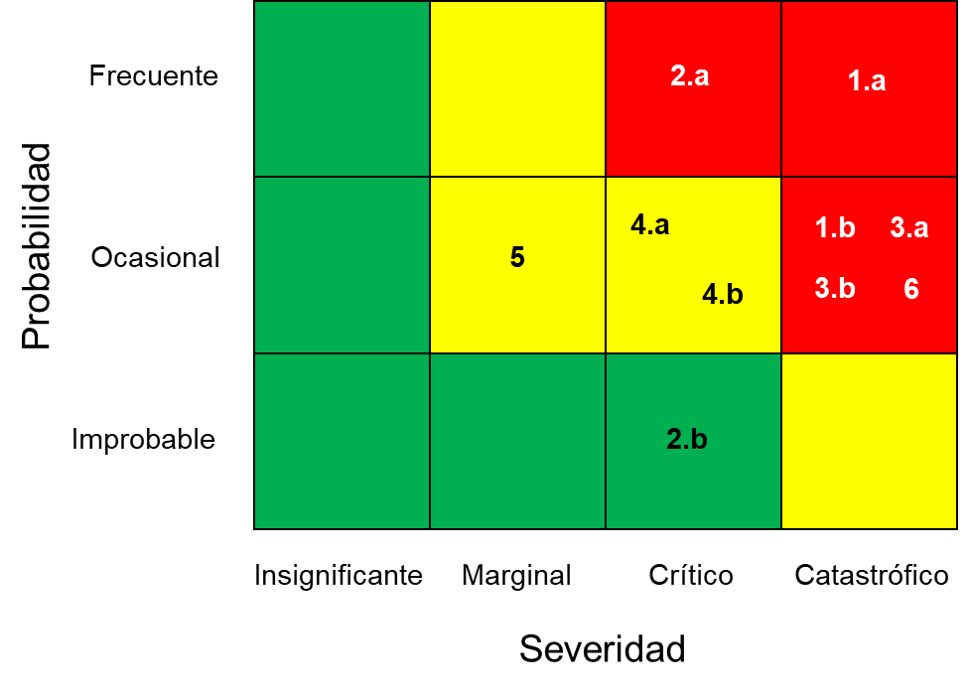
\includegraphics[width=0.5\paperwidth,keepaspectratio]{matriz_riesgo.png}
\end{center}
\caption{Matriz de Riesgo}
\end{figure}

\end{document}
